\section{Reducing preparation failures}
\label{sec:preparation}
The shared-model result separates two costs that require different changes. Its supplied-basis calls complete, while some initial reference calculations or enlarged-region checks fail. We therefore change the preparation workflow and train a second model on individual successful and failed attempts. This comparison includes basis lookup or discovery, both exact reductions, prediction, recovery, and process exit.

The compact workflow first looks for previously checked master indices with the same ordered propagator structure and zero-mass pattern. It reuses these indices while recomputing all coefficients at the new kinematic values. Without a stored basis, it begins with a compact seed region and treats the resulting basis as provisional. A second reduction uses that basis and a different integral ordering, and its coefficients must agree exactly. Kira's supplied-basis check rejects additional masters~\cite{Kira3}. Agreement checks the requested reductions; it does not prove that the provisional basis has the globally smallest possible number of masters. Incomplete attempts expand the seed region, and duplicate attempts are removed.

The new model takes the same 44 structural quantities as the neural model, together with the three seed bounds, the truncation flag and level, the presence and size of a supplied basis, and the integral-ordering setting. Its 52 inputs predict log attempt time and a failure score. We fit random forests and extremely randomized forests~\cite{Breiman2001Forest,Geurts2006ExtraTrees} and select the action with the smallest sum of predicted time and a validation-selected failure penalty. Appendix~\ref{app:risk} defines the outputs and objective. The failure score ranks actions; it is not a calibrated probability.

Training uses 1,405 earlier attempts, including 389 failures, and 58 separate validation requests select the model. The selected random forest has 32 trees of maximum depth 6 and uses a 120-second failure penalty. Fitting and model selection take 3.67 seconds, excluding the earlier cost of collecting labels. Training includes the initial shared-model trial, but excludes the distinct-mass vacuum family, nonplanar boxes, pentagons, and loop orders six and above. The new physical profile supplies no fitting or selection labels.

The reserved comparison contains 33 requests at one through seven loops, using the physical definitions in Appendix~\ref{app:families-new} with profile $h=1237$. It compares expanded discovery and its enlarged-region check with three versions of the compact workflow: native bounds, the frozen neural model, and the cost-and-risk model. Each method receives the same 110-second request deadline and a 60-second cap per native call. Every first attempt is retained, and each initially successful method receives two further repetitions. All four methods use the same 128-bit integral-ordering labels, which Kira supports~\cite{Kira3}; this setting changes the internal ordering representation rather than the exact coefficient arithmetic. The 31-coordinate interface limit remains.

\begin{table}[!htbp]\centering\small
\caption{Preparation outcomes over the full reserved set. The first-pass timer includes successful and unsuccessful requests. Failed-attempt time counts the unsuccessful native calls within that pass. These totals describe work performed; a shorter failed request is not a successful speedup.}
\label{tab:preparation-coverage}
\begin{tabularx}{\linewidth}{@{}Yrrrr@{}}\toprule
Method & First complete & All 3 complete & First pass (s) & Failed calls (s)\\\midrule
Expanded discovery & 17/33 & 16/33 & 1041.6 & 684.2\\
Compact, no ML & 23/33 & 23/33 & 757.8 & 573.1\\
Compact, neural model & 23/33 & 23/33 & 869.0 & 663.4\\
Compact, cost and risk & 23/33 & 23/33 & 895.1 & 677.6\\
\bottomrule\end{tabularx}\end{table}

\begin{table}[!htbp]\centering\small
\caption{Preparation completions by loop order. Each entry requires all three repetitions. The compact columns use the same reuse and checking procedure with the stated decision rule. These results are separate from the earlier supplied-basis coverage in Table~\ref{tab:general-coverage}.}
\label{tab:preparation-loops}
\begin{tabular}{@{}rrrrrr@{}}\toprule
Loops & Requests & Expanded & Compact native & Neural & Cost and risk\\\midrule
1 & 4 & 4 & 4 & 4 & 4\\
2 & 7 & 6 & 7 & 7 & 7\\
3 & 4 & 3 & 3 & 3 & 3\\
4 & 6 & 2 & 3 & 3 & 3\\
5 & 6 & 1 & 4 & 4 & 4\\
6 & 4 & 0 & 2 & 2 & 2\\
7 & 2 & 0 & 0 & 0 & 0\\
\bottomrule\end{tabular}\end{table}

\begin{table}[!htbp]\centering\small
\caption{Complete preparation time on matched requests. Every included method completes all three repeats in the same master-index basis with exact coefficient agreement. The compact/native comparison includes reuse and the changed check; the two ML comparisons isolate prediction within that workflow.}
\label{tab:preparation-times}
\begin{tabularx}{\linewidth}{@{}Yrrr@{}}\toprule
Comparison & Matched & Time ratio & Repeat interval\\\midrule
Compact without ML / expanded & 13 & 0.305 & [0.290,0.329]\\
Neural model / compact without ML & 22 & 0.982 & [0.959,1.021]\\
Cost and risk / compact without ML & 22 & 1.635 & [1.604,1.700]\\
Cost and risk / neural model & 23 & 1.536 & [1.471,1.595]\\
\bottomrule\end{tabularx}\end{table}

The analysis performs 6,375 coefficient comparisons across the repeated and competing outputs. The reused index cache contains 24 earlier checked structures. Their retained discovery and check records cost 341.3 seconds before this experiment; failed attempts during the earlier search add further cost. The compact timings therefore describe use of an existing cache, not cost-free master discovery. In the earlier supplied-basis experiment, 129 neural-model native attempts contain 0 failures. This audit locates the larger failure cost in preparation.

\begin{figure}[!htbp]\centering
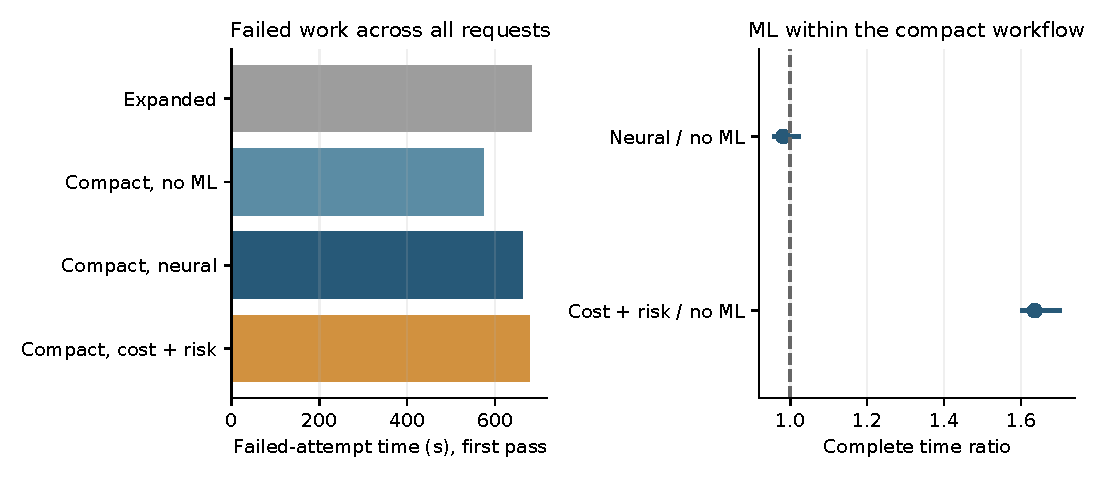
\includegraphics[width=\linewidth]{paper_figures/preparation_results.pdf}
\caption{The preparation comparison keeps failed work and the added ML effect separate. The left panel includes failed calls from every first request. The right panel uses only exact matched completions and compares both models with the same compact workflow without ML. The dashed line marks equal time.}
\label{fig:preparation}
\end{figure}
\FloatBarrier

Compact preparation without ML compared with expanded discovery gives ratio 0.305 on 13 matched requests, with repeat interval [0.290,0.329]. The neural model within compact preparation gives ratio 0.982 on 22 matched requests, with repeat interval [0.959,1.021]. The cost-and-risk model within compact preparation gives ratio 1.635 on 22 matched requests, with repeat interval [1.604,1.700]. The cost-and-risk model increases time in this broad comparison. The neural preparation result also remains consistent with equal time. We keep the failure model and its records for analysis, while the shared neural model remains the validated supplied-basis default.

The full application first checks whether the restricted scalar massless formula applies. This is a physical condition, independent of measured time. Among the remaining requests, the neural preparation model gives ratio 0.985 on 21 matched completions, with repeat interval [0.963,1.025], relative to compact preparation without ML. These measurements do not meet both conditions for retaining learned preparation: a time interval below one and completion of every request completed by its native control. The default therefore uses native choices for preparation and retains the shared neural model for supplied-basis reduction, where the separate test establishes a gain. This deployment choice follows the candidate comparisons. The reported ratios belong to the frozen methods; they do not provide a new independent timing test of the resulting selector.

\subsection{Recovery from an incomplete stored basis}
The first compact trial exposed a target-dependent basis mismatch: a basis checked for earlier targets can omit masters needed by a new batch. The revised application discards a rejected cached basis after expanded seeding also fails, rediscovers without that constraint, and checks the result. It also permits an expanded target check when smaller checks fail. All steps remain inside the same 110-second request budget. A focused follow-up uses six fresh requests at two through five loops and keeps the models and index cache fixed. All three repetitions complete on 6/6 requests with ML disabled, 6/6 with the neural model, and 6/6 with the cost-and-risk model. The neural model gives a ratio of 0.783 on 6 matched requests, with repeat interval [0.743,0.797], relative to the revised workflow without ML. The cost-and-risk model gives a ratio of 0.801 on 6 matched requests, with repeat interval [0.772,0.857], relative to the revised workflow without ML. The comparison passes 2,352 coefficient checks. It tests the recovery change on fresh parameters of selected structures and does not replace the broad trial.
